\documentclass[12pt]{article}

% Packages
\usepackage{amsmath}
\usepackage{graphicx}
\usepackage{booktabs}
\usepackage{natbib}
\usepackage{hyperref}
\usepackage{geometry}
\usepackage{mathptmx} % Times font
\usepackage{multirow}
\usepackage{array}
\usepackage{placeins}

% Page setup
\geometry{margin=1in}

% Hyperref setup
\hypersetup{
  colorlinks=true,
  linkcolor=blue,
  citecolor=blue,
  urlcolor=blue
}

\title{Trajectory Dynamics in Language Model Hidden States Predict Human Processing Costs Beyond Surprisal}

\author{Elan Barenholtz\\
Machine Perception \& Cognitive Robotics Laboratory\\
Department of Psychology / Center for Complex Systems\\
Florida Atlantic University\\
\texttt{elan.barenholtz@fau.edu}}

\date{}

% ---- REVIEW AID: new/changed text in v2 is wrapped in \new{...} and set bold.
% ---- To turn the highlighting off, change the definition to \newcommand{\new}[1]{#1}
\newcommand{\new}[1]{#1}   % highlighting off for submission (set to {\bfseries #1} to mark v2 changes)

\begin{document}

\maketitle

\begin{abstract}
Language comprehension is necessarily sequential. Each word arrives against a context created by the words before it, and that context is continually changing. Surprisal---the negative log probability of a word given its context---has become the dominant way of relating this incremental process to processing time. Yet surprisal throws away almost all of the structure in the underlying representation. It tells us how unexpected a word was, but not whether that word continued the direction in which the representation had been moving or pushed it somewhere else. A dynamical view of comprehension suggests that this distinction may matter. It is also plausible from the production side: speakers generally plan over short stretches, so natural language may contain local directional continuity over a few words. We test this with a simple measure, trajectory extrapolation error. At each word, we fit a line through the preceding hidden states of a transformer language model, extrapolate that line one step, and ask how far the actual state lands from that extrapolated point. On the Natural Stories corpus, this measure is \new{correlated with but not reducible to} surprisal (\new{$r = .31$}) and independently predicts self-paced reading times. The effect \new{survives a control built from four surprisal estimates spanning GPT-2 and Pythia and replicates across model scale and} across architectures with different positional encoding schemes (GPT-2 vs.\ Pythia/RoPE). \new{In a second self-paced corpus of 2,000 participants the effect is present in the same direction but falls short of our pre-specified reliability criterion on participant sign agreement (61\%, against a threshold of 65\%); we report it as partial rather than full replication.} A displacement control shows the effect is not reducible to representational change magnitude\new{: entered together, extrapolation error retains its effect and displacement does not}. \new{Neither extrapolation error nor surprisal accounts for the magnitude of garden-path difficulty at the item level, consistent with prior benchmark findings.} The results point to two partly separable sources of \new{self-paced reading} cost: how unexpected the word is, and how much it breaks with the local direction of the evolving representation.

\end{abstract}

\newpage

\section{Introduction}

Language comes in a sequence. The reader or listener never gets the whole sentence at once; each word modifies an interpretation that is already underway. Word-by-word reading time gives us a fairly direct behavioral trace of that process. One of its most robust features is also one of the simplest: predictable words tend to be read faster than unpredictable ones. The dominant computational framework for explaining this regularity is surprisal theory \citep{hale2001,levy2008}, which holds that the cost of processing a word is proportional to its negative log probability given the preceding context. % [v2] DELETED: the v1 sentence beginning "The framework follows naturally from
% information-theoretic considerations..." committed to a belief-updating
% mechanism (comprehender maintains a probability distribution; low-probability
% words impose an update cost). Removed rather than rewritten.
Surprisal predicts reading times across self-paced reading \citep{smith2013}, eye-tracking \citep{demberg2008}, and neural measures \citep{frank2015}.

Surprisal is only as useful as the model used to estimate it. Early work relied on n-gram models and probabilistic grammars \citep{hale2001,demberg2008,roark2009}, which provided useful but limited estimates of word predictability. Transformer-based language models have since become the standard tool \citep{goodkind2018,wilcox2020,schrimpf2021}, largely because their surprisal estimates are better predictors of human reading times than those from earlier models, and because they can condition on arbitrarily long contexts rather than fixed windows. There is another reason they are useful here. They are themselves sequential processors: trained to predict the next token given the preceding sequence, they build rich internal representations that update incrementally as each word is encountered. Because these models are trained on human-produced text, the statistical structure they capture --- sensitivity to context, coherence, discourse --- is the same structure latent in that production, which is what makes their surprisal a useful index of the predictive regularities to which human comprehenders are sensitive.

Still, prediction is not the only way to think about a sequential process. An alternative theoretical tradition treats comprehension not as a series of independent predictions but as a dynamical process in which the interpretive state evolves through a continuous representational space \citep{tabor1999,spivey2007,cho2017}. On this view, it matters not only where the interpretive state is at a given moment, but how it got there and where it appears to be going. This is especially likely for language, because human language production itself is a sequential, locally planned process. Speakers and writers plan a few words ahead, execute that plan, and then re-plan \citep{levelt1989,ferreira2002}, creating text with local momentum: stretches over which the context evolves in a coherent direction before shifting. If this momentum is a real property of natural language, and if comprehenders are sensitive to it, then the direction in which the interpretation has been evolving, not just the probability of the next word, should matter for processing.

To test this idea we need some representation in which an evolving trajectory can actually be measured. Transformer language models such as GPT-2 \citep{radford2019} provide one. Their hidden states encode a rich, incrementally updated representation of the context processed so far, and because the model is trained on human-produced text, these representations come to reflect not only the predictive structure that surprisal captures, but also other latent regularities of production --- including the short-horizon continuity of how each word's representation extends from those of its predecessors. Here, we introduce a simple measure that we call trajectory extrapolation error. At each word position, we fit a linear trajectory to the hidden states of the preceding $k$ words (typically $k = 3$), extrapolate one step forward, and measure the Euclidean distance between this predicted position and the actual hidden state. The measure captures the degree to which the current word deviates from where the representation was heading: high extrapolation error means the representation was moving in one direction and the current word forced it somewhere else; low error means the current word continued the established drift.

The comparison with surprisal is deliberately one-sided. Surprisal is expected to predict processing cost under either tradition, since improbable words tend to disrupt trajectories; finding that surprisal matters does not distinguish between the frameworks. What would be informative is the reverse result: trajectory extrapolation error explaining variance that surprisal leaves behind. it would suggest that the dynamical character of comprehension contributes to processing cost in a way that word-level prediction error does not capture. Two words with identical conditional probability receive identical surprisal even if one continues an established interpretive trajectory and the other forces a sharp representational turn, and any cost difference between such words is evidence for directional dynamics in comprehension. This asymmetry is not a limitation of the language models from which surprisal is derived: their hidden states already carry the trajectory information, but surprisal as an output measure collapses it to a scalar.

\new{The question, then, is whether the information discarded by surprisal has any measurable relation to human processing.} Human processing unfolds under strong constraints of recency and local influence \citep{gibson1998,lewis2005}, meaning that recent words dominate the current interpretive state. Under such constraints, the trajectory of the interpretation over the last few words is the comprehender's best available signal about where things are heading. A reader who is sensitive to that recent drift could use it as a cheap summary of where the interpretation is headed. That does not require treating every word as an independent prediction problem. Garden-path sentences provide an intuitive illustration: in ``The horse raced past the barn fell,'' each word after ``raced'' reinforces the main-verb interpretation, building momentum in one direction, and the cost at ``fell'' reflects not just the word's unexpectedness but the reversal of accumulated interpretive direction. But if trajectory sensitivity is a general feature of human processing, the phenomenon should not be limited to garden paths. Any word that forces the interpretation off its recent trajectory should incur a cost, even in ordinary text, and this cost should be measurable independently of surprisal.


\new{Our primary dataset is the Natural Stories corpus \citep{futrell2018}, where the measure can be evaluated over thousands of word positions of naturalistic connected text read by 181 participants. This is the larger and less constrained test, and it is where our analytic decisions---the model specification, the use of subject-level inference, and the criteria for judging an effect reliable---were made. We then turn to the Classic Garden Path materials of the SAP Benchmark \citep{huang2024}, carrying those decisions over. The control set is not identical across the two corpora: connected text and 13--17 word isolated sentences require position to be handled differently, and the sentence corpus uses distance from sentence start and end with quadratic terms in place of the running-text position and previous-reading-time controls. The inferential criteria, the measure, and the model form are unchanged. These materials were of interest for a specific reason: the disambiguating word of a garden-path sentence is a theoretically motivated locus of trajectory disruption, a point at which the interpretation is known to reverse, and if the measure indexes the cost of such reversals it should register there in particular. We ask two questions of them. The first concerns the ambiguity manipulation: does the difference in extrapolation error between a garden-path sentence and its unambiguous control predict the difference in reading time, across items? The second sets the manipulation aside and treats the materials as what they also are---a second self-paced reading corpus, 144 syntactically difficult sentences read by 2,000 participants---and asks whether the Natural Stories result holds there.}

\new{Both corpora use self-paced reading, which delivers words serially, one at a time and only on request. We take up the question of whether the effect extends to reading with free eye movements separately; the evidence reported here concerns serial presentation.}

Three additional analyses clarify what the measure captures. A displacement control assesses whether the contribution of extrapolation error reduces to the magnitude of representational change at each word. A direction-preservation analysis on the Natural Stories corpus characterizes the temporal scale of the underlying trajectory structure in the model. Finally, \new{a cross-architecture replication using Pythia (which uses Rotary Position Embeddings rather than the absolute positional embeddings of GPT-2) tests whether any effect of trajectory structure generalizes across model scale and positional encoding scheme, and a series of surprisal controls drawn from larger models tests whether the effect is a residual of poor predictability estimation by any one model}.

\section{Method}

\subsection{Materials}

\paragraph{Garden-path sentences.} To test the trajectory effect at a controlled, theoretically motivated locus of disruption, we used the Classic Garden Path subset of the SAP Benchmark \citep{huang2024}, a large-scale syntactic ambiguity processing dataset. The subset contains 24 items covering three structural types: main-verb/reduced-relative (MVRR; e.g., ``The horse raced past the barn fell''), NP/S direct-object/sentential-complement (e.g., ``The suspect showed the file deserved more attention''), and NP/Z transitive/intransitive (e.g., ``While the man hunted the deer ran into the woods''). Each item appeared in ambiguous and unambiguous conditions, where the unambiguous version included an overt syntactic marker (e.g., a relative pronoun) that prevents the garden-path misparse. Human reading-time data were collected via self-paced word-by-word reading from over 2,000 participants. Reaction times were filtered to exclude responses below 100 ms or above 5,000 ms.\new{\footnote{An earlier version of this paper (arXiv:2606.05346v1) reported a reading-time analysis restricted to the critical region of these materials. That analysis contained a sample-construction error and is withdrawn; see the version note. The materials are analysed here in two ways: as an ambiguity manipulation at the item level, and as a corpus of connected text.}} \new{These sentences were presented in isolation rather than embedded in running text, so fit windows near the start of a sentence could in principle include the first token, whose hidden-state magnitude is anomalously large in transformer models \citep{xiao2023}. We therefore begin every fit window at the second token, which excludes that position by construction and restricts the analysis to word positions 5 and later.}

\paragraph{Natural Stories.} To evaluate the same measure across thousands of word positions in naturalistic text, we used the Natural Stories corpus \citep{futrell2018}, which consists of 10 naturalistic narratives totaling approximately 10,000 words. Self-paced reading times were collected from 181 participants, yielding \new{848,875} observations after filtering to 100--3,000 ms\new{; 813,621 remain after merging to the measure sample, and 812,730 from 178 participants enter the fitted models once the previous-word control is defined}. We processed each story through GPT-2 in overlapping chunks to accommodate the model's 1,024-token context limit, computing hidden states and surprisal at every word position.

\subsection{Trajectory Extrapolation Error}

\paragraph{Definition.} Let $h_t$ denote the hidden-state vector at word position $t$ in a given layer of a transformer language model. For a window of size $k$, we fit a linear trajectory to the hidden states at positions $t{-}k$ through $t{-}1$ by ordinary least squares. The extrapolated position at the next time step is the linear prediction at time $k$, and trajectory extrapolation error is defined as the Euclidean distance between the extrapolated and actual hidden states (see Figure~\ref{fig:schematic} for a schematic illustration). This quantity measures how far the representation landed from where it was heading, given the trajectory established by the preceding $k$ words.

\begin{figure}[!ht]
\centering
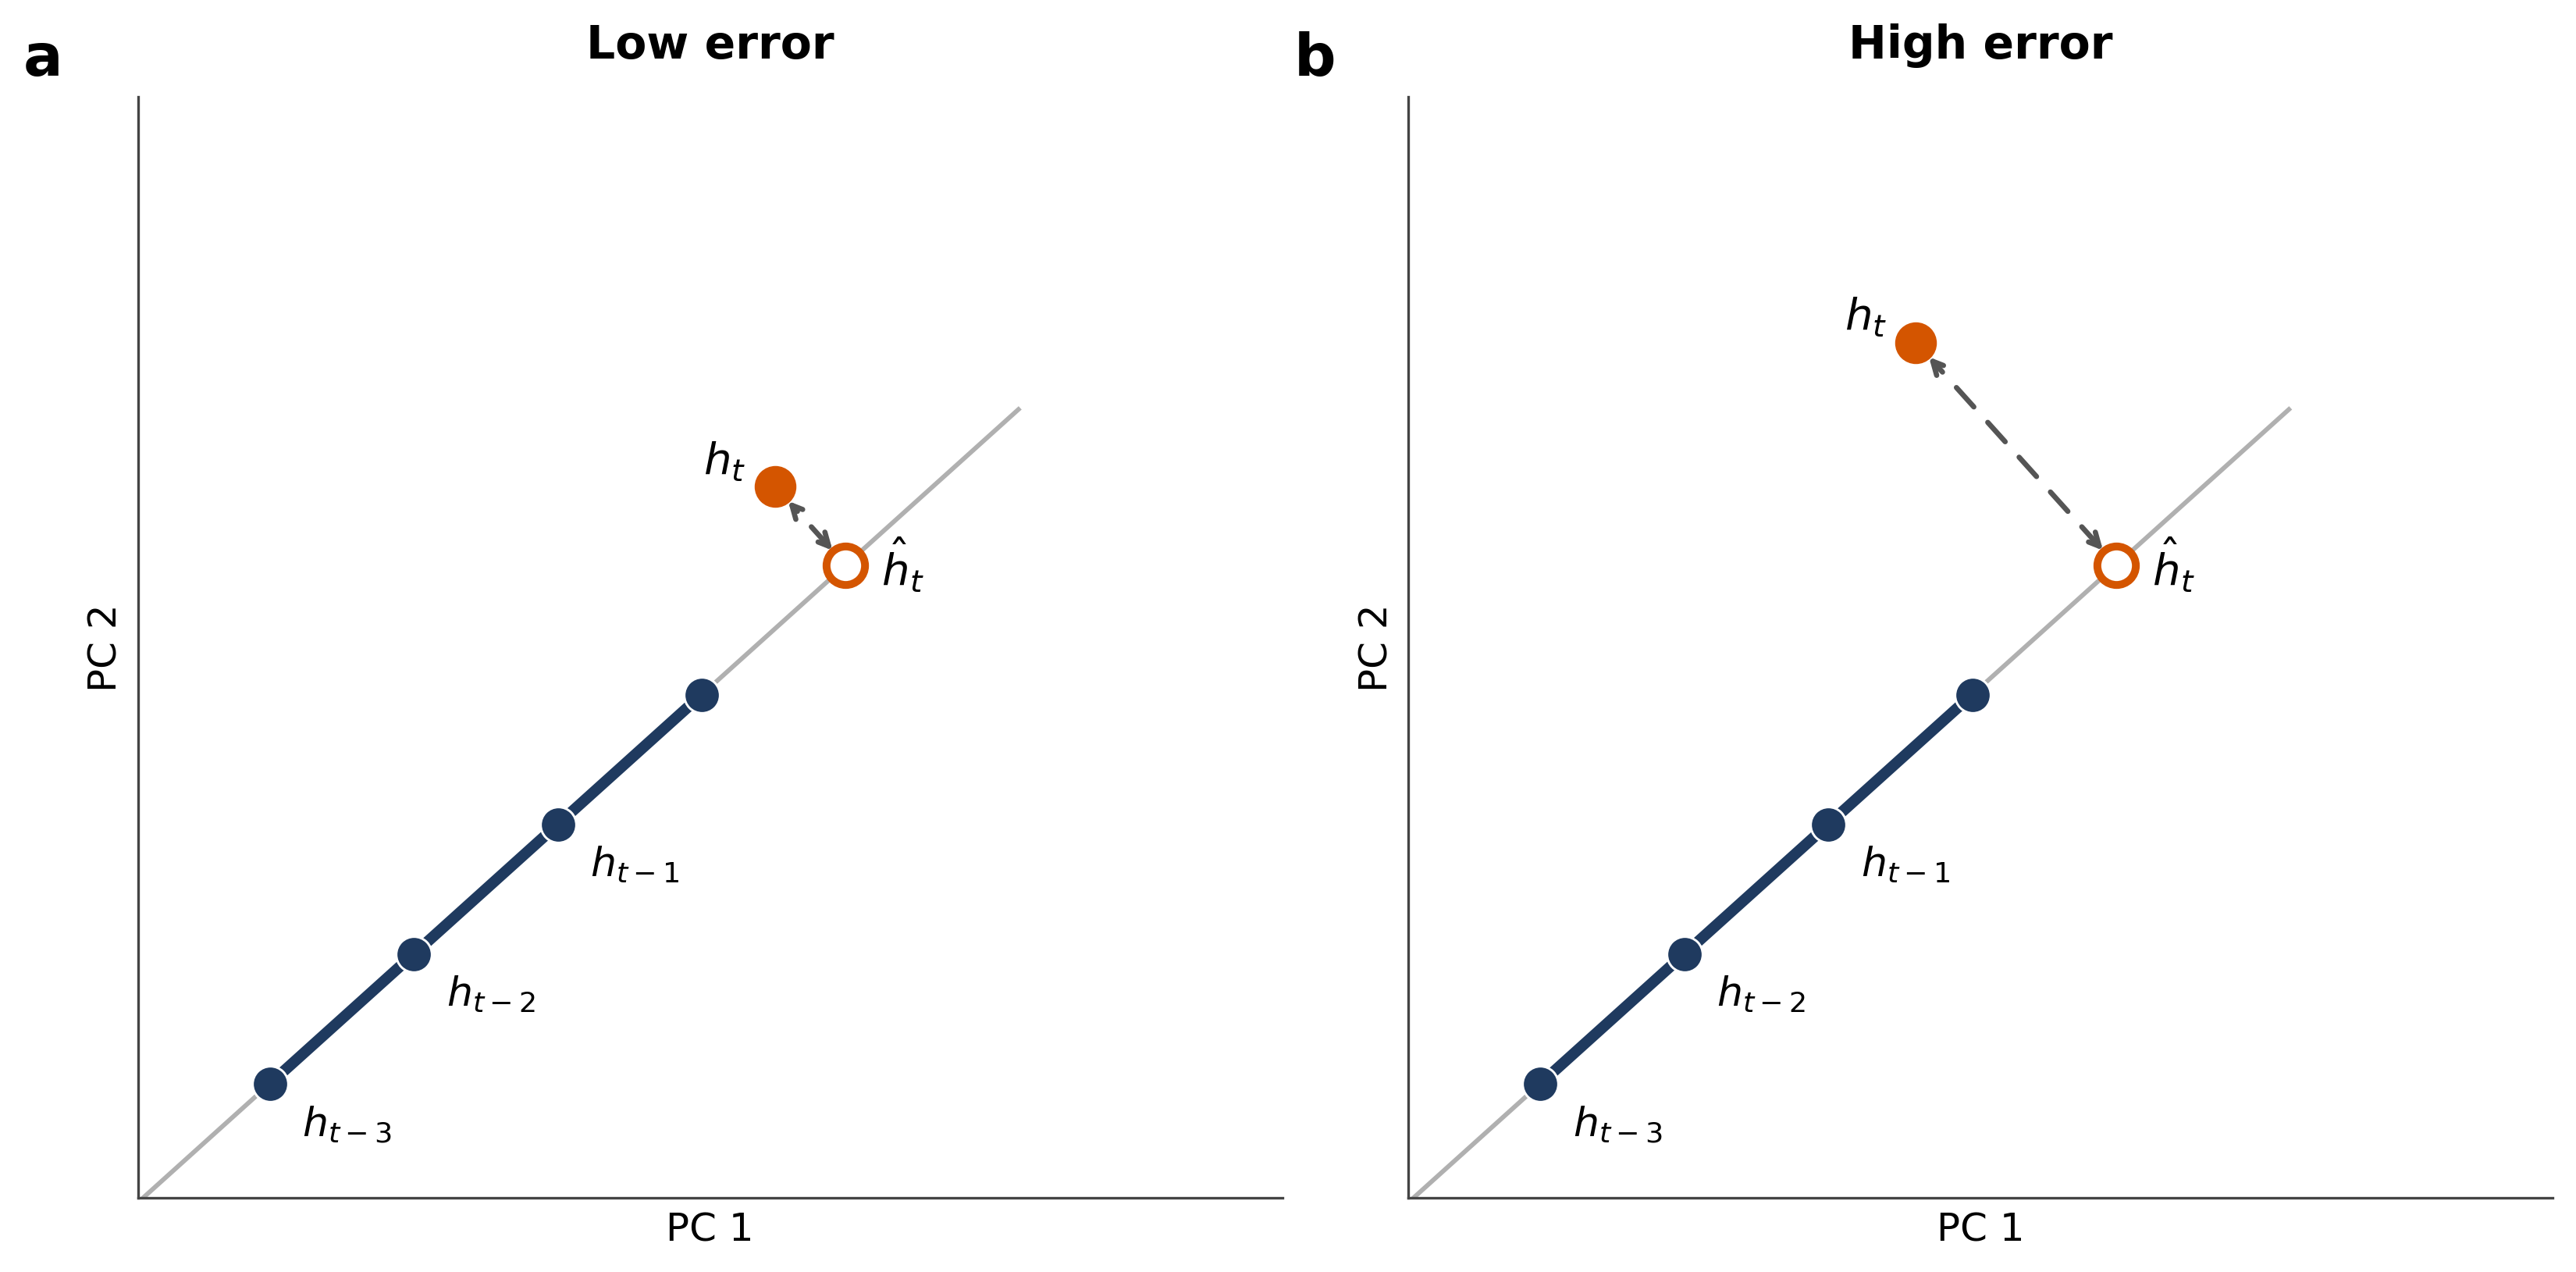
\includegraphics[width=\textwidth]{fig1_schematic.png}
\caption{Schematic illustration of trajectory extrapolation error. Each point $h_t$ represents the model's hidden-state vector at word position $t$, projected into a two-dimensional principal-component space for visualization. A linear trajectory is fit to the hidden states at the preceding $k$ positions (here $k = 3$: $h_{t-3}$ through $h_{t-1}$) and extrapolated one step forward to produce a predicted position (open circle, $\hat{h}_t$). Trajectory extrapolation error is the Euclidean distance between this predicted position and the actual hidden state $h_t$ (filled orange circle). (a) Low error: the current word's hidden state falls near the extrapolated position, continuing the established trajectory. (b) High error: the current word (e.g., a garden-path disambiguator) forces the hidden state far from the extrapolated position.}
\label{fig:schematic}
\end{figure}

\paragraph{Parameter selection.} We computed extrapolation error using GPT-2 (117M parameters; \citealp{radford2019}), which sits near the sweet spot for reading-time prediction identified by \citet{oh2023a}. We tested two layers: layer 6 (an intermediate layer) and the final layer (layer 12). We focus primarily on layer 6 because intermediate layers are known to capture syntactic representations more effectively than output layers in transformer models \citep{hewitt2019,jawahar2019}. \new{The 3-word window and layer 6 were fixed in the previous version of this work and are retained here unchanged. We report the window sweep on the corrected pipeline for transparency, because it does not favour that choice: entered in the headline specification, $k = 2$ improves fit by $\Delta\text{AIC} = 539.6$ ($\beta = +0.0072$, 84.2\% of participants positive) and $k = 7$ by $85.5$, against $78.4$ for the reported $k = 3$. Fit degrades from $k = 15$ and reverses sign by $k = 30$. We do not adopt the best-fitting window, because selecting the parameter on the outcome variable is precisely the researcher degree of freedom this paper is otherwise at pains to avoid; $k = 3$ is retained for continuity with the earlier report. A reader should treat the window as a fixed prior choice rather than an optimised one, and note that the measure at $k = 2$---the discrete second difference of the hidden-state sequence---is a different quantity that merits separate investigation. Layer and polynomial-degree variants are not present in the locked sample and were not re-verified under the corrected pipeline.} For sentences with subword tokenization, we used the hidden state at the last subword token of each word.

\subsection{Direction Preservation Analysis}

To characterize the trajectory structure underlying extrapolation error, we computed a direction preservation measure on the Natural Stories corpus. At each word position, we measured the absolute cosine similarity between the fitted trajectory direction (from the preceding $k$ words) and the actual displacement vector at the current word and at 1, 2, and 3 steps ahead. The question is simply whether the direction of change at one position carries over to the positions that follow. For random vectors in 768-dimensional space, the expected absolute cosine similarity is approximately 0.029, providing a chance baseline.

\subsection{Statistical Analyses}

We fit linear mixed-effects models predicting log-transformed reading times, with random intercepts for participants. All continuous predictors were $z$-scored prior to entry. \new{Word frequency is the Zipf value of the lowercased word with attached punctuation removed. We note this explicitly because the frequency values used in v1 were derived without that normalisation and were zero for 19.7\% of tokens, including ordinary words carrying attached punctuation and words differing only in case; all frequency-dependent analyses reported here have been recomputed.} The baseline model (M0) included word length, word position, previous log RT, and log word frequency (Zipf score; standard psycholinguistic control, e.g., \citealp{smith2013}) as lexical controls. We then tested a series of nested models: M1 added surprisal; M2 added trajectory extrapolation error. Model comparisons were evaluated using the Akaike Information Criterion (AIC), the Bayesian Information Criterion (BIC), and likelihood ratio tests. AIC estimates out-of-sample prediction error, with lower values indicating better fit; BIC applies a stronger penalty for model complexity and is more conservative. For the Natural Stories analysis, we additionally included log word frequency as a control and tested the independence of surprisal and extrapolation error via correlation and a tercile-based dissociation analysis. As a further control, we tested whether extrapolation error reduces to simple one-step representational change by comparing it with embedding displacement ($\|h_t - h_{t-1}\|$) in a joint model including both measures alongside surprisal and lexical controls.

\new{Because a pooled model over hundreds of thousands of observations can register an effect that no individual reader shows, the headline reading-time analyses in both corpora were additionally estimated separately within each participant and tested across participants. We treat an effect as reliable when the group-level test reaches $p < .01$ and at least 65\% of participants share the sign of the coefficient. These criteria were fixed on Natural Stories and applied unchanged thereafter. Where sign agreement is reported, it is accompanied by a permutation floor obtained by shuffling the measure within participant and refitting.}

\new{To test the robustness of the effect across model scale and architecture, we repeated the Natural Stories analysis using Pythia-160M and Pythia-410M \citep{biderman2023}, which use Rotary Position Embeddings rather than the learned absolute position embeddings of GPT-2, testing the proportionally equivalent mid-layer of each. All models were evaluated on identical rows and identical participants.}

\new{Two comparisons were run on the garden-path materials. The first treats them as an ambiguity manipulation: for each item we computed the ambiguous-minus-unambiguous difference in extrapolation error, in surprisal, and in mean log reading time at the disambiguating word, and asked whether the model-derived differences predict the behavioural one across items, with and without fixed effects for construction. The second sets the manipulation aside and treats the materials as a reading-time corpus, using the same specification developed on Natural Stories.}

\section{Results}

\new{Figure~\ref{fig:contrib} gives the main result up front. In both self-paced corpora, trajectory extrapolation error accounts for
reading-time variance that surprisal and lexical frequency do not, at roughly a
third the magnitude of surprisal in Natural Stories and comparably to it in the
garden-path corpus. The evidence is stronger in Natural Stories, which meets our
pre-specified reliability criterion; the garden-path corpus does not, and is
reported as a partial replication. The sections below establish that result on the Natural
Stories corpus, carry the same measure, inferential procedure and reliability
criterion over to the garden-path materials with corpus-appropriate nuisance
controls, and
then examine what the measure is and is not capturing.}

\subsection{Natural Stories}

\new{\paragraph{Reading-time prediction.} Trajectory extrapolation error predicts self-paced reading time beyond surprisal and lexical controls ($\Delta\text{AIC} = 78.4$, $\beta = +0.0030$, $p = 3.1 \times 10^{-19}$, $N = 812{,}730$, 178 participants). For comparison, in the same model $\beta(\text{surprisal}) = +0.0103$, $\beta(\text{word length}) = +0.0134$ and $\beta(\text{log frequency}) = +0.0045$: the trajectory effect is a little under a third the magnitude of surprisal, and is a second-order effect on reading time rather than a competitor to it (Figure~\ref{fig:contrib}).}

\new{\paragraph{Subject-level inference.} Because a pooled model over 812,730 observations can register an effect that no individual reader exhibits, we estimated the model separately within each participant. Of 171 participants with sufficient data, 115 (67.3\%) showed a positive coefficient (sign test $p = 7.6 \times 10^{-6}$; Wilcoxon $p = 2.4 \times 10^{-9}$; $t(170) = 6.74$). Thirty-two participants reached individual significance. We adopt this form of inference throughout, and take 65\% sign agreement together with a group-level $p < .01$ as the criterion for a reliable effect.}

\new{\begin{figure}[!htbp]
\centering
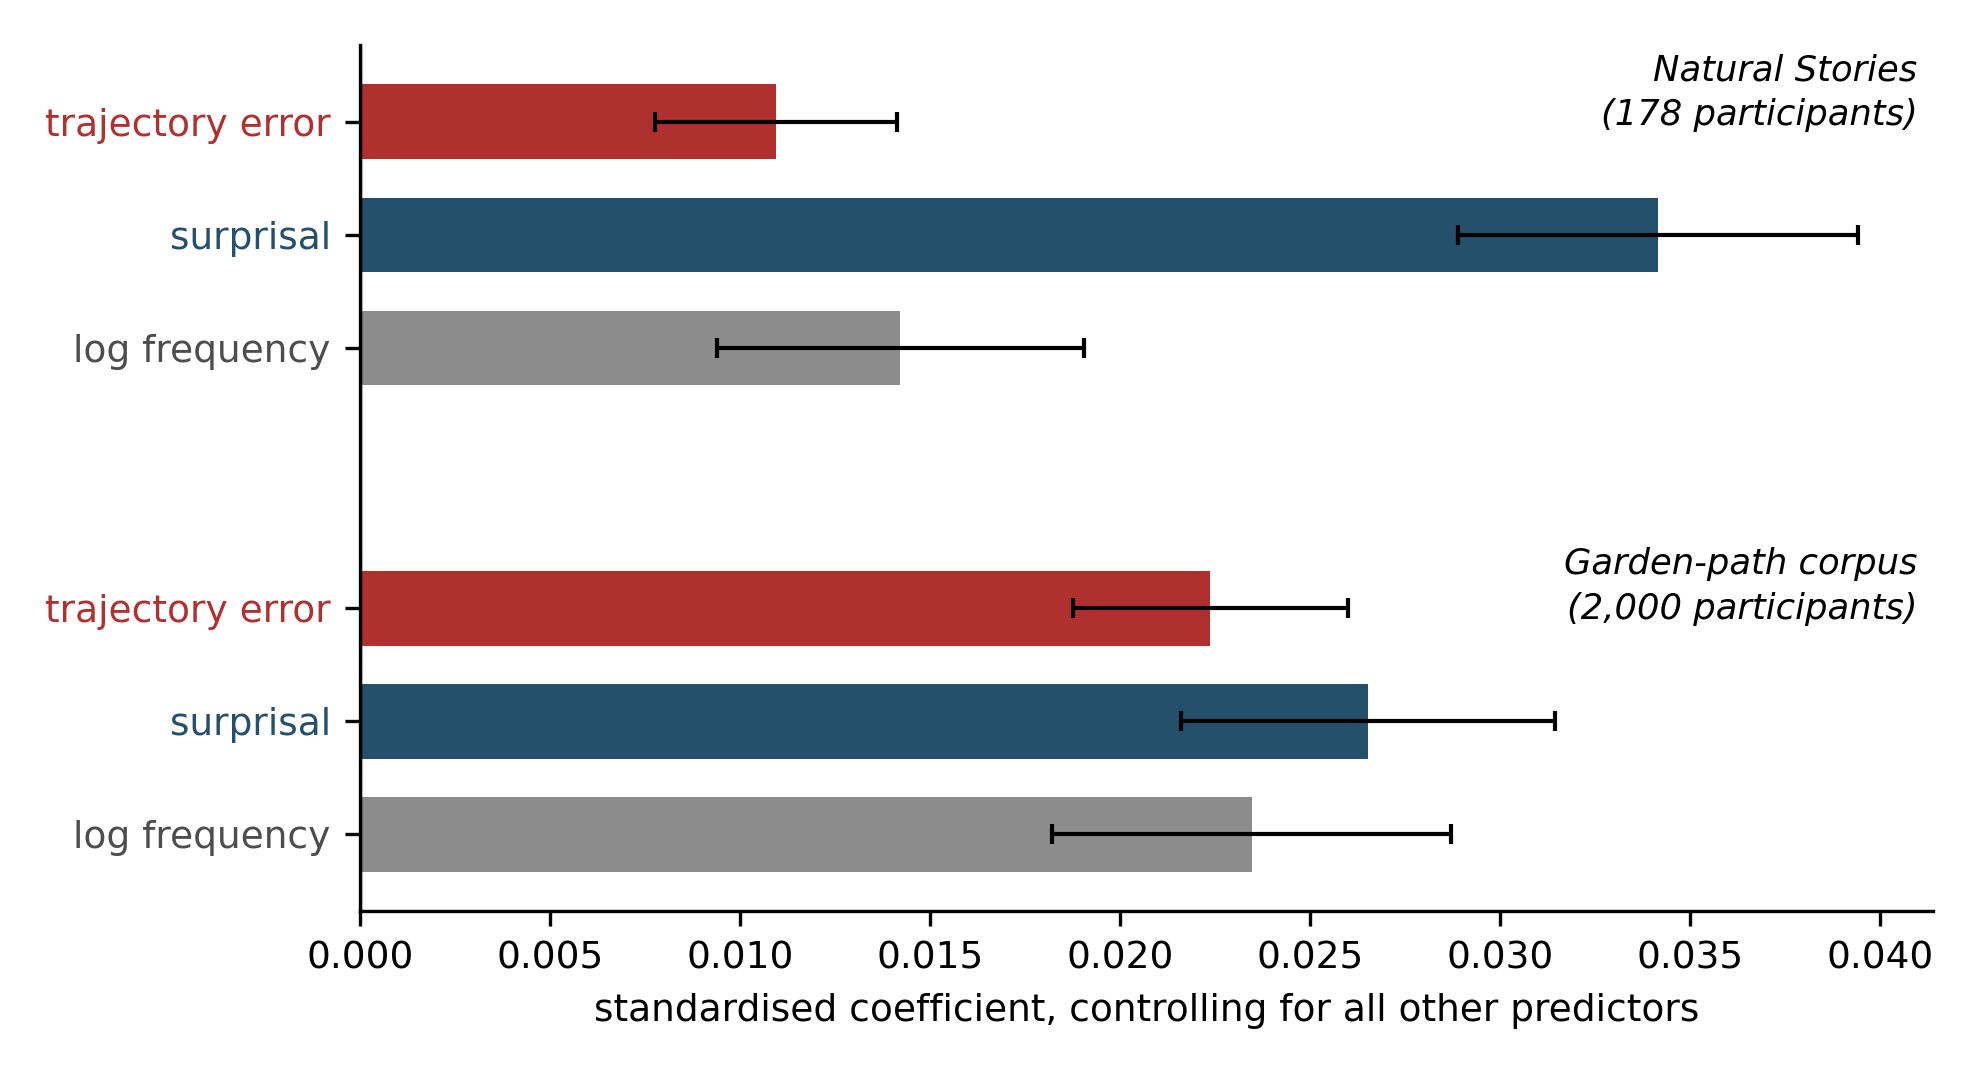
\includegraphics[width=0.72\textwidth]{fig_core.png}
\caption{Unique contribution of each predictor to self-paced reading time, in
both corpora. Each coefficient is estimated within participant with every other
predictor in the model, and averaged across participants; bars are 95\%
confidence intervals over participants. Trajectory extrapolation error accounts
for reading-time variance that surprisal and lexical frequency do not, at
roughly a third the size of surprisal in Natural Stories and comparably to it in
the garden-path corpus. Nuisance controls are included in every model but omitted from the plot; these
differ by corpus, being previous reading time and linear sentence position for
Natural Stories, and distance from sentence start and end with quadratic terms
for the garden-path corpus; word length is likewise omitted, being large enough in the garden-path
corpus ($+0.135$) to compress the remaining bars. Coefficients are standardised
within participant, so magnitudes are not directly comparable across corpora.}
\label{fig:contrib}
\end{figure}}

\new{\paragraph{Robustness.} The effect survives a control for word identity, centring the outcome and the remaining predictors within word type (2,919 types occurring five or more times; word length and frequency are constant within type and therefore drop out): it attenuates substantially but remains ($\Delta\text{AIC} = 23.1$, $p = 5.3 \times 10^{-7}$). A substantial share of the raw effect is therefore lexical, and a trajectory-specific component survives. Adding a punctuation covariate reduces it ($\Delta\text{AIC} = 70.0$), while restricting to punctuation-free words strengthens it ($\Delta\text{AIC} = 114.9$, $\beta = +0.0038$, $n = 716{,}641$).}

\paragraph{Independence of measures.} \new{The next question is what, exactly, separates the two measures.} The correlation between surprisal and extrapolation error at the word level was \new{$r = .31$, indicating that the two measures share roughly ten percent of their variance}. Whatever trajectory extrapolation error captures, it is not a nonlinear transformation of surprisal. \new{Because the measures are correlated, the evidence that each contributes independently rests on the analyses below rather than on the correlation.}

\paragraph{Dissociation analysis.} We split words into terciles on both surprisal and extrapolation error and examined mean log reading times in each cell of the resulting $3 \times 3$ matrix (Table~\ref{tab:dissociation}; Figure~\ref{fig:dissociation}). Words with high surprisal but low extrapolation error (surprising words that continue the trajectory) showed an increase of \new{$+0.029$} in log RT over the low/low baseline (\new{$t = 14.38$, $p = 8 \times 10^{-47}$}). Words with low surprisal but high extrapolation error (unsurprising words that disrupt the trajectory) showed an increase of \new{$+0.010$} (\new{$t = 5.43$, $p = 6 \times 10^{-8}$}). Both effects are significant. So the dissociation is present in both directions.

\paragraph{Regression.} A mixed-effects model containing both $z$-scored surprisal and $z$-scored extrapolation error gave the same basic result: independent\new{, additive contributions from each ($\beta_{\text{surprisal}} = +0.0102$, $\beta_{\text{extrapolation}} = +0.0030$). The additive model was preferred over one including their interaction ($\Delta\text{AIC} = 1.5$ in favour of the simpler model; interaction $\beta = +0.0002$, $p = .49$), indicating that surprisal and extrapolation error combine without amplifying or dampening each other. The margin is small, and we would not read the additivity as established, but there is no evidence of interaction.}

\begin{table}[!htbp]
\centering
\caption{Dissociation Matrix: Mean Log Reading Time by Surprisal $\times$ Extrapolation Error Tercile (Natural Stories)}
\label{tab:dissociation}
\begin{tabular}{lccc}
\toprule
 & \textbf{Low extrap error} & \textbf{Mid extrap error} & \textbf{High extrap error} \\
\midrule
\textbf{Low surprisal} & \new{baseline} & \new{+0.005} & \new{+0.010} \\
\textbf{Mid surprisal} & \new{+0.016} & \new{+0.016} & \new{+0.028} \\
\textbf{High surprisal} & \new{+0.029} & \new{+0.031} & \new{+0.041} \\
\bottomrule
\end{tabular}

\smallskip
\footnotesize
\textit{Note.} \new{Values are differences in mean log reading time from the low-surprisal / low-extrapolation baseline (5.717).} Off-diagonal cells represent the key dissociation: high surprisal / low extrapolation error reflects surprise without trajectory disruption; low surprisal / high extrapolation error reflects trajectory disruption without surprise. Both off-diagonal effects are independently significant (see text).
\end{table}

\begin{figure}[!htbp]
\centering
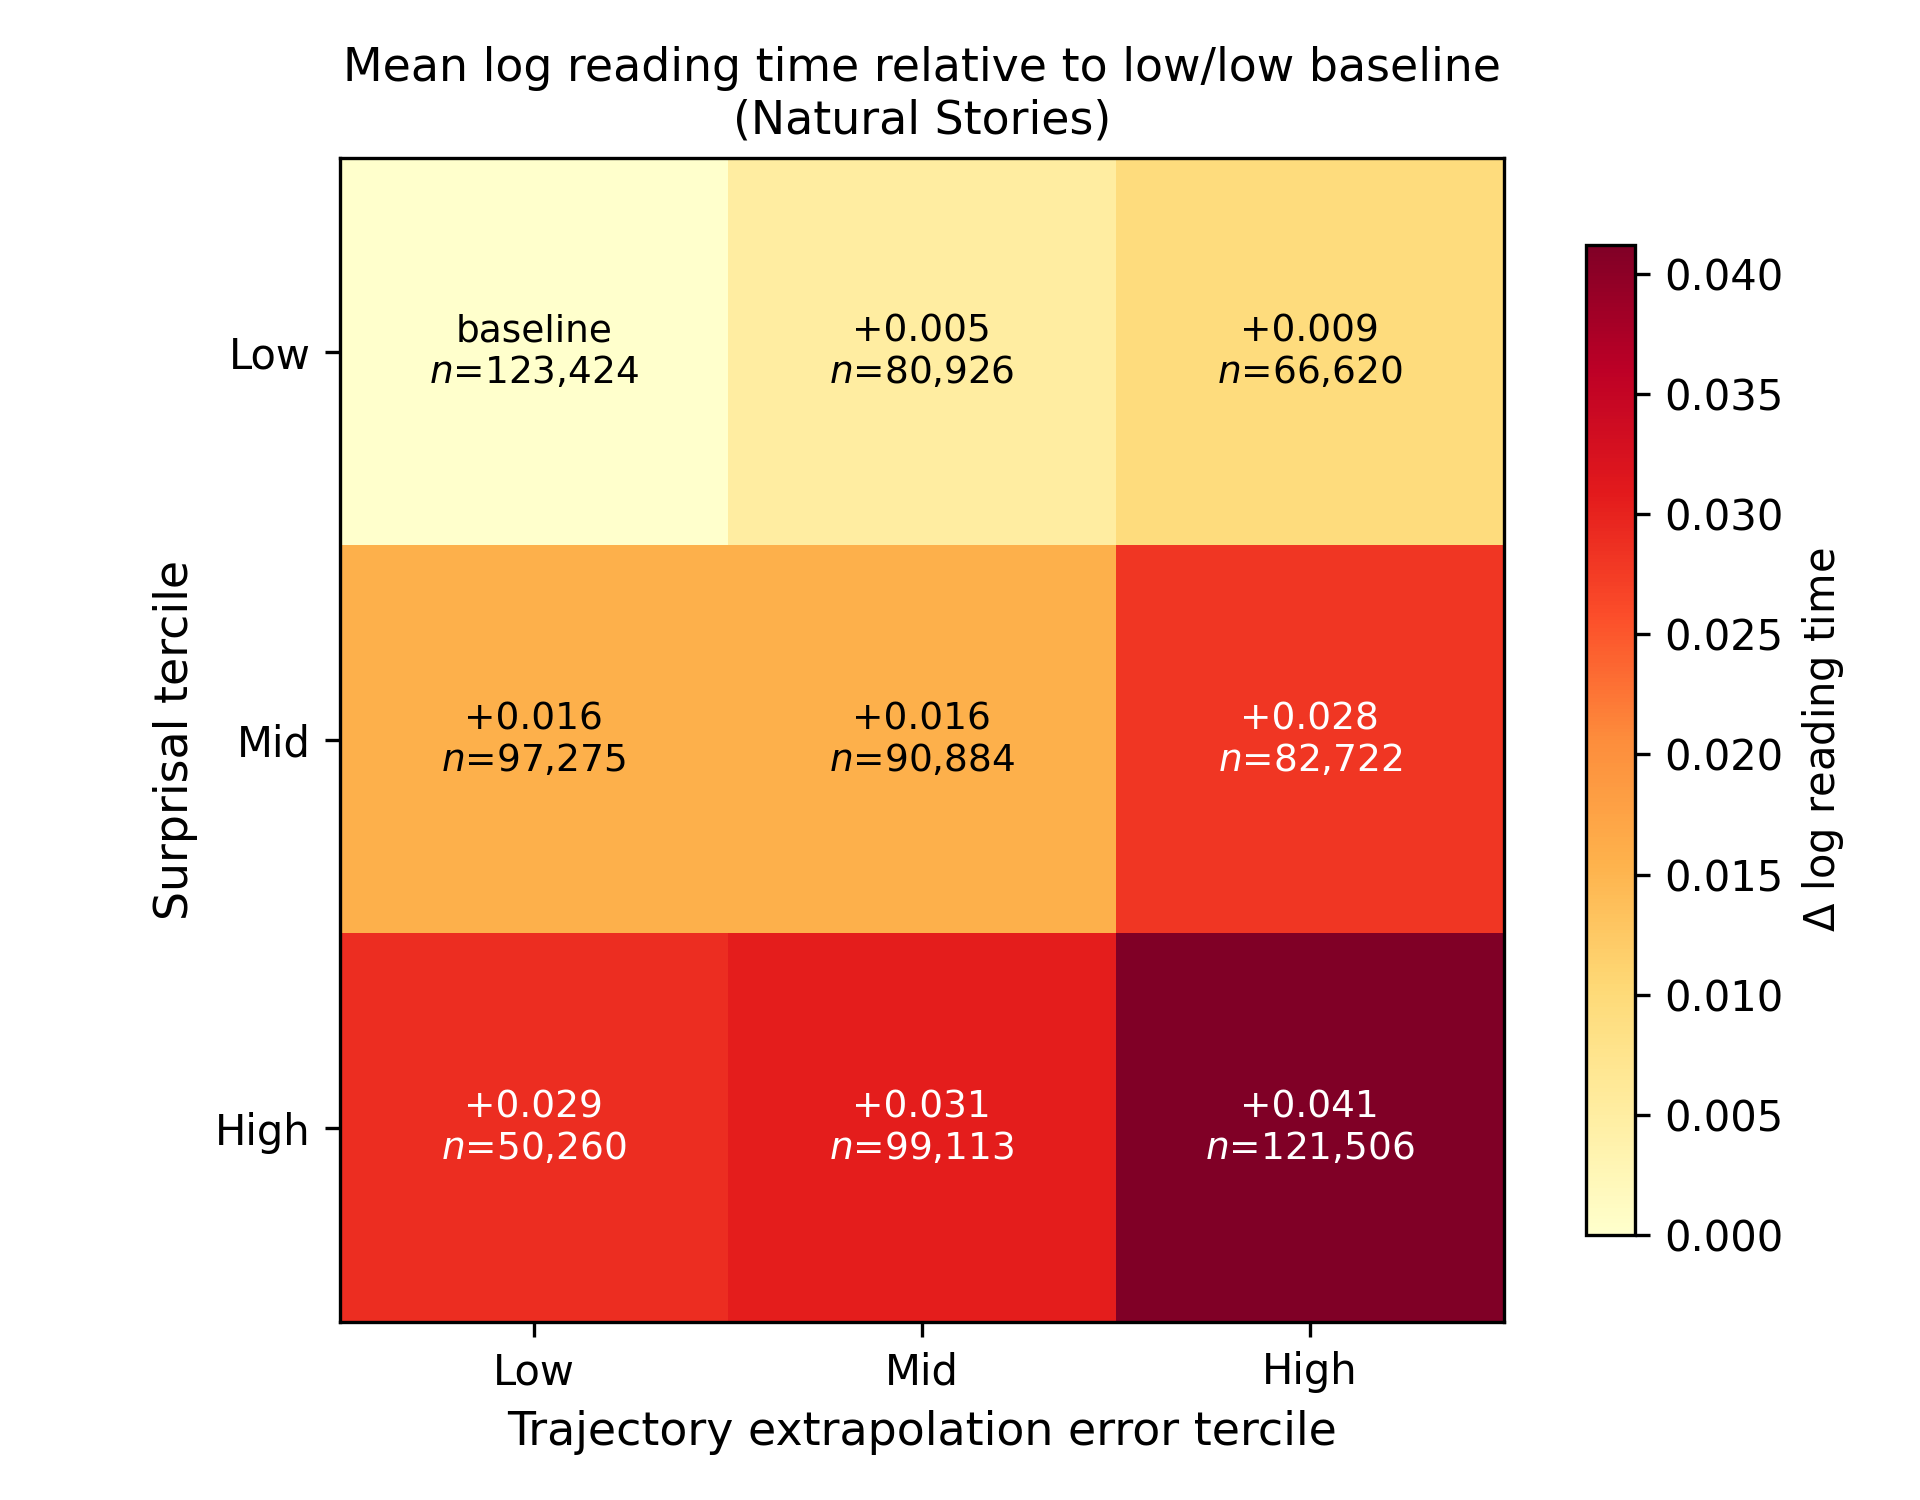
\includegraphics[width=0.8\textwidth]{fig3_dissociation.png}
\caption{Dissociation between surprisal and trajectory extrapolation error in Natural Stories. Heatmap shows mean log reading time in each cell of the $3 \times 3$ tercile matrix. The off-diagonal cells demonstrate that each measure captures unique variance: high surprisal / low extrapolation error (surprise without trajectory disruption) and low surprisal / high extrapolation error (trajectory disruption without surprise) both produce elevated reading times relative to the low/low baseline.}
\label{fig:dissociation}
\end{figure}

\FloatBarrier

\new{\subsection{Garden-Path Materials}

\paragraph{The ambiguity contrast.} Extrapolation error at the disambiguating word is higher in ambiguous than unambiguous sentences for NP/S ($+2.55$, 20 of 24 items) and NP/Z items ($+4.25$, 23 of 24), but reverses for main-verb/reduced-relative items ($-1.72$, 17 of 24, $t(23) = -3.26$, $p = .003$). Surprisal does not reverse for these items ($+5.23$, 23 of 24). The reversal reflects the item set rather than the measure. At the disambiguating word the three constructions produce nearly identical extrapolation error in the ambiguous condition (99.2, 98.3, 99.1), but the MV/RR unambiguous control sits at 101.0 against 95.7 and 94.8 for the other two. That control restores a full passive relative clause (``the horse \emph{that was} raced past the barn fell''), a low-frequency and structurally heavy construction that perturbs the trajectory about as much as the garden path does, so the difference score for these items compares two disrupted states rather than a disrupted state against a baseline. The disambiguating word and the three words entering its fit window are identical across conditions, so the difference is carried entirely by earlier context.

\paragraph{Item-level prediction.} Neither measure predicts the size of the human garden-path effect. Across 72 item $\times$ construction pairs, the ambiguous-minus-unambiguous difference in extrapolation error does not predict the corresponding difference in reading time once construction is controlled ($\beta = -0.019$, $p = .89$); surprisal does no better ($\beta = -0.035$, $p = .78$). This is the same basic failure reported by \citet{huang2024} on these materials.

\paragraph{Reading-time prediction across the corpus.} Setting the ambiguity manipulation aside, these 144 sentences constitute a self-paced reading corpus of syntactically difficult material read by 2,000 participants, and we analysed it as such: all words, all conditions, no region selection. Words whose fit window is undefined are excluded, restricting the analysis to word positions 5 and later and leaving 444,737 observations. Estimating the model separately within each participant and testing the coefficients across participants, extrapolation error predicted log reading time with word length, log frequency, punctuation, and position within the sentence entered flexibly (distance from sentence start and end, each with a quadratic term): $\beta = +0.0224$, 61.1\% of participants positive, Wilcoxon $p = 2.7 \times 10^{-32}$. Adding a sentence-final indicator to absorb wrap-up effects strengthens it slightly ($\beta = +0.0251$, 62.7\%). Permuting the measure within participant and refitting gives 50.7\% sign agreement (pooled over ten shuffles, range 49.5--51.9\%), which is the baseline against which those values should be read. The corresponding floor in Natural Stories is 48.8\% (range 45.6--57.3\%; the wider spread reflects the smaller participant sample). Entering the trajectory term as a B-spline rather than linearly does not improve fit in either corpus ($\Delta$AIC $-0.5$ to $-4.6$ in Natural Stories and $-2.0$ to $-6.8$ in the garden-path corpus, for 3 to 8 degrees of freedom), so we report it linearly throughout.

Replacing linear surprisal with a spline leaves the estimate essentially unchanged ($df = 3$: $+0.0202$; $df = 5$: $+0.0207$; $df = 8$: $+0.0209$). Read from the same per-participant fits, extrapolation error is the more consistent of the two measures across participants (61.1\% against surprisal's 56.6\%) but the smaller in magnitude: within participants $|\beta(\text{extrapolation})|$ exceeded $|\beta(\text{surprisal})|$ in 42.1\% of cases (paired $p = 3.7 \times 10^{-21}$). As in Natural Stories, it is a second-order contribution alongside surprisal rather than a competitor to it.

A threshold of 65\% sign agreement was fixed in advance of these analyses, carried over from Natural Stories. Neither measure meets it here under flexible position controls. Participants in this corpus contribute roughly 220 observations each against thousands in Natural Stories, so per-participant coefficients are correspondingly noisy, and we report sign agreement descriptively against the permutation floor rather than as a criterion.

\paragraph{Stronger surprisal controls.} Because the trajectory measure and the surprisal control are both derived from GPT-2 Small, the effect could in principle mark the words at which that model's probability estimate is poor rather than any property of the trajectory; controlling for the same model's surprisal cannot remove such a confound. Substituting surprisal from GPT-2 XL ($\beta = +0.0255$) or Pythia-410M ($+0.0255$), entering all three together ($+0.0254$), or splining all three at $df = 4$ ($+0.0246$) leaves the estimate unchanged. The same holds in Natural Stories, where the effect survives GPT-2 Medium ($\Delta\text{AIC} = 90.7$), GPT-2 XL ($95.7$) and Pythia-410M ($87.9$) surprisal entered singly, and all four jointly ($82.1$), against $78.4$ for the original specification.}

\subsection{Displacement Control}

To test whether extrapolation error reduced to simple representational change, we compared it with one-step displacement, $\|h_t - h_{t-1}\|$. \new{The two measures are strongly correlated ($r = .80$), and each predicts slower reading when entered alone (extrapolation error $\beta = +0.0030$; displacement $\beta = +0.0021$). Entered jointly with surprisal and lexical controls, however, extrapolation error retains its effect and in fact strengthens ($\beta = +0.0033$, $p = 2.8 \times 10^{-11}$), while displacement contributes nothing ($\beta = -0.0005$, $p = .35$; Table~\ref{tab:displacement}). Given how strongly the measures correlate, that result is useful: what predicts reading time is not representational movement as such, but the component of that movement which departs from the established trajectory. At least for this control, the effect cannot be reduced to the magnitude of representational change alone.}

\begin{table}[!htbp]
\centering
\caption{Displacement Control: Joint Model of One-Step Displacement and Extrapolation Error on Natural Stories Reading Times}
\label{tab:displacement}
\begin{tabular}{lrrr}
\toprule
\textbf{Predictor} & $\boldsymbol{\beta}$ & $\boldsymbol{\chi^2(1)}$ & $\boldsymbol{p}$ \\
\midrule
\new{Extrapolation error, alone} & \new{$+0.0030$} & \new{---} & \new{$3.1 \times 10^{-19}$} \\
\new{Displacement, alone} & \new{$+0.0021$} & \new{---} & \new{---} \\
\new{Extrapolation error, joint} & \new{$+0.0033$} & \new{---} & \new{$2.8 \times 10^{-11}$} \\
\new{Displacement, joint} & \new{$-0.0005$} & \new{---} & \new{$.35$} \\
\bottomrule
\end{tabular}

\smallskip
\footnotesize
\textit{Note.} \new{Mixed-effects models with by-participant random intercepts, alongside surprisal and lexical controls; $n = 812{,}730$. Correlation between displacement and extrapolation error: $r = .80$. Entered jointly, extrapolation error retains its effect and displacement falls to non-significance.}
\end{table}

\subsection{Direction Preservation}

The layers behave quite differently (Table~\ref{tab:direction}; Figure~\ref{fig:direction}). At layer 6, direction preservation at the current word position is 0.44, well above the random baseline of 0.029. However, preservation drops to 0.10 at one step ahead and remains at approximately 0.08 for two and three steps ahead. \new{Direction preservation falls sharply after a single word, to roughly a fifth of its value at the current step.} At the final layer, direction preservation at the current step is 0.61 and remains at 0.54 across one, two, and three steps ahead. The final layer maintains persistent directional structure that the intermediate layer does not.

This also changes how the layer-6 measure should be interpreted. \new{Because direction preservation falls sharply after one step}, the linear fit over 3 words does not capture a persistent trajectory; rather, it captures local positional continuity --- the smooth displacement of hidden states due to the incremental nature of contextual updating.

\begin{table}[!htbp]
\centering
\caption{Direction Preservation in Natural Stories by Layer and Steps Ahead}
\label{tab:direction}
\begin{tabular}{lccccc}
\toprule
\textbf{Layer} & \textbf{Current step} & \textbf{+1 step} & \textbf{+2 steps} & \textbf{+3 steps} & \textbf{Random baseline} \\
\midrule
Layer 6 ($w = 3$) & \new{0.436} & \new{0.099} & \new{0.078} & \new{0.077} & 0.029 \\
Layer 12 ($w = 3$) & \new{0.615} & \new{0.541} & \new{0.540} & \new{0.539} & 0.029 \\
Layer 6 ($w = 5$) & \new{0.396} & \new{0.097} & \new{0.076} & \new{0.073} & 0.029 \\
Layer 12 ($w = 5$) & \new{0.602} & \new{0.547} & \new{0.543} & \new{0.544} & 0.029 \\
\bottomrule
\end{tabular}

\smallskip
\footnotesize
\textit{Note.} Values represent mean absolute cosine similarity between the fitted trajectory direction and the displacement vector at each word position. Random baseline is the expected absolute cosine similarity between random vectors in 768-dimensional space.
\end{table}

\begin{figure}[t]
\centering
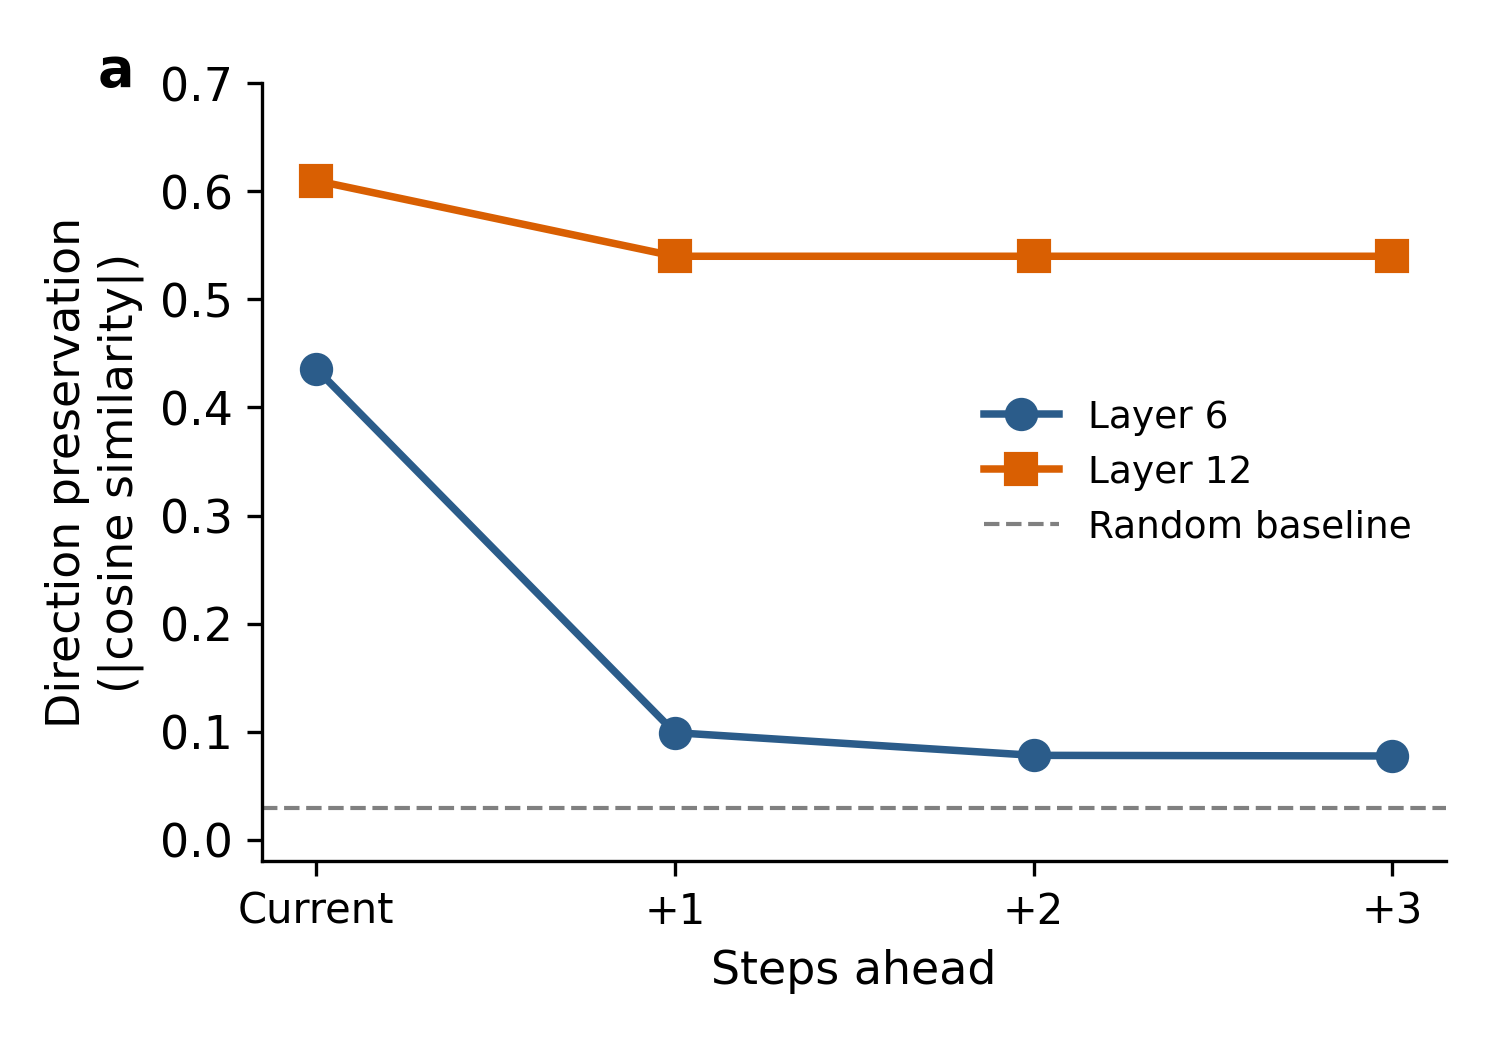
\includegraphics[width=0.8\textwidth]{fig4_direction.png}
\caption{Direction preservation decay by layer and steps ahead (Natural Stories). At layer 6, direction preservation drops from 0.44 at the current step to 0.10 at one step ahead, close to but above the random baseline, indicating that directional structure decays rapidly. At the final layer (layer 12), direction preservation remains elevated (0.54) across all steps ahead, indicating persistent directional structure. Dashed horizontal line indicates the random baseline for 768-dimensional vectors (0.029).}
\label{fig:direction}
\end{figure}

\subsection{\new{Model Scale and Architecture}}

Up to this point the analyses use GPT-2 variants, all of which share an architecture and learned absolute positional embeddings. To test whether the trajectory extrapolation effect depends on this specific positional encoding scheme, we replicated the Natural Stories analysis using Pythia models \citep{biderman2023}, which use Rotary Position Embeddings (RoPE), a fundamentally different approach that encodes position through rotation of the hidden-state vectors rather than through additive position embeddings. We tested Pythia-160M (comparable to GPT-2 Small; mid-layer 6 of 12) and Pythia-410M (comparable to GPT-2 Medium; mid-layer 12 of 24).

The same basic effect appears in both Pythia models (Table~\ref{tab:crossarch}). \new{All three models were evaluated on identical rows and identical participants ($n = 812{,}730$, 178 participants). Trajectory extrapolation error predicted reading times beyond surprisal in both Pythia-160M ($\Delta\text{AIC} = 88.3$, $\beta = +0.0029$, $p = 2.0 \times 10^{-21}$) and Pythia-410M ($\Delta\text{AIC} = 400.2$, $\beta = +0.0065$, $p = 1.7 \times 10^{-89}$), against $78.4$ for GPT-2 Small on the same data.} Direction preservation showed the same rapid decay at the mid-layer, dropping from 0.42 to near-random levels within a single step for both Pythia models, confirming that the \new{rapid decay of directional structure} is not an artifact of GPT-2's coordinate system.

\begin{table}[!htbp]
\centering
\caption{Cross-Architecture Replication: Pythia (RoPE) vs.\ GPT-2 (Absolute Position Embeddings)}
\label{tab:crossarch}
\begin{tabular}{lccrcc}
\toprule
\textbf{Model} & \textbf{Pos.\ enc.} & \new{$\boldsymbol{\beta}$} & \textbf{$\Delta$AIC} & \textbf{Dir.\ pres.\ +0} & \textbf{Dir.\ pres.\ +1} \\
\midrule
GPT-2 Small (117M) & Absolute & \new{$+0.0030$} & \new{78.4} & 0.44 & 0.10 \\
Pythia-160M & RoPE & \new{$+0.0029$} & \new{88.3} & 0.42 & 0.13 \\
Pythia-410M & RoPE & \new{$+0.0065$} & \new{400.2} & 0.42 & 0.11 \\
\bottomrule
\end{tabular}

\smallskip
\footnotesize
\textit{Note.} $\Delta$AIC extrap / surprisal = improvement from adding trajectory extrapolation error to the model already containing surprisal and lexical controls. \new{All three models are evaluated on identical rows and identical participants ($n = 812{,}730$, 178 participants).} Direction preservation values are mean absolute cosine similarity between the fitted trajectory direction and the displacement vector at the current (+0) and next (+1) word positions.
\end{table}

\FloatBarrier

\section{Discussion}

\subsection{Two Dimensions of Sequential Processing}

Surprisal has been enormously useful for predicting incremental processing cost. But it is still one number per word. Whatever is happening in the underlying representation gets collapsed into that number. The results here suggest that some of what gets lost in that collapse is related to reading time. There seem to be two separable pieces: how unlikely the word is in context, and how far the new representation departs from the local path established over the preceding few words. The trajectory effect \new{is strong in Natural Stories, appears in the same direction but only partially replicates in a second self-paced reading corpus, and is also present across} architectures with very different positional encoding schemes (GPT-2's absolute embeddings and Pythia's Rotary Position Embeddings). That makes a coordinate-system artifact difficult to sustain as the explanation.

Surprisal and trajectory extrapolation error are \new{correlated but far from redundant ($r = .31$ in Natural Stories)}, and both contribute to reading time. That is a little striking because they come from the same model on the same words. But they are asking different questions. Surprisal asks how unlikely the word was given the full context. Extrapolation error asks whether the hidden state landed roughly where its recent motion would have put it. Those can come apart. A word can be quite predictable and still redirect the representation; another can be unlikely but continue the local drift. The \new{dissociation matrix shows a reading-time cost in both off-diagonal cases}.

\new{This does not mean that either measure resolves the standing difficulties for surprisal-based accounts. \citet{huang2024} report that language model surprisal does not explain the magnitude of syntactic disambiguation difficulty, with garden-path constructions showing the largest misalignment. Our item-level analysis of their materials reproduces this. Across 72 item $\times$ construction pairs, the ambiguous-minus-unambiguous difference in surprisal does not predict the corresponding difference in reading time once construction is controlled ($\beta = -0.035$, $p = .78$), and extrapolation error does no better ($\beta = -0.019$, $p = .89$). Moving from a model's output probabilities to the geometry of its internal states does not repair that misalignment.}

\new{There is a methodological wrinkle here. Surprisal from larger, lower-perplexity language models is a \textit{weaker} predictor of human reading times \citep{oh2023b}, so substituting a larger model's surprisal makes for a less stringent control rather than a more stringent one: it absorbs less of the outcome variance, and any predictor entered alongside it will appear correspondingly stronger. We therefore evaluate extrapolation error against a control containing all four surprisal estimates entered together.}

The displacement control analysis in GPT-2 rules out the simplest alternative interpretation of the trajectory-extrapolation error finding: that it merely indexes the magnitude of representational change in the embedding space. \new{The two measures are strongly correlated ($r = .80$) and each predicts slower reading alone, but entered together only extrapolation error retains an effect; displacement contributes nothing. What predicts reading time is therefore not representational movement as such, but the component of that movement which departs from the established trajectory.} However, the core finding, that trajectory extrapolation error contributes to reading-time prediction beyond surprisal, is robust across architectures.

The Natural Stories effect is not large. Its coefficient is modest, and surprisal accounts for much more. Still, the effect is useful because it survives controls that should absorb several simpler explanations. \new{There is also an important failure. The measure does not become especially informative at the point where the motivating intuition is strongest: the disambiguating word in a garden-path sentence. Neither extrapolation error nor surprisal predicts which garden-path items produce the larger human cost. So whatever extrapolation error is tracking, these data do not justify identifying it with garden-path reanalysis itself.} The narrower conclusion is that word-by-word reading time contains a small component related to short-horizon representational continuity that is not captured by surprisal.

I would not take this as evidence for a long, smooth trajectory through sentence space. In fact, the direction-preservation result argues against that picture. At the predictive layer the direction largely disappears after a single step. What the reading-time effect seems to track is much more local: continuity over a few neighboring states. That is a weaker claim than a general dynamical theory of comprehension, but it is also the claim the data actually support.

\subsection{Trajectory as a Functional Property of Language}

Why should there be local trajectory structure in language in the first place? Production offers one plausible source. Speaking and writing are locally planned: a few words are prepared, produced, and then the plan is updated \citep{levelt1989,ferreira2002}. That should leave some short-range continuity in the signal. A phrase develops, a clause develops, a topic carries for a bit, and then something changes. I do not think the present data let us identify the three-word window with a literal production-planning window. That would be too neat. But the match in timescale is at least suggestive, and it gives a concrete reason that local directional structure might be present in ordinary text.

The model, of course, was never trained to preserve trajectories. If this structure appears in its hidden states, the straightforward explanation is that next-word prediction forced the model to absorb regularities that are already present in human-produced text. The direction-preservation analysis also puts an important limit on this story. At the predictive layer, directional persistence is nearly gone after one step. So the model contains local geometry that can be measured as a trajectory, but there is no evidence here that the model itself is explicitly extrapolating that trajectory as a processing strategy.

Humans also do not have unlimited access to the full preceding context. Processing is recency-weighted and working memory is limited \citep{gibson1998,lewis2005}. Some compressed representation of recent context has to do a lot of work. A local trajectory is one possible summary: not a record of everything that came before, just an indication of where the interpretation has recently been going. The present result is consistent with readers being sensitive to something of that sort. It does not show that they literally fit or extrapolate a line in a representational space.

Garden paths give the clearest intuition for what a trajectory break might look like. The local trajectory established by the ambiguous region points in the wrong direction, and the disambiguating word reveals that what looked like a coherent local trajectory was misleading. \new{That intuition motivated the measure, but the item-level analysis does not bear it out: neither extrapolation error nor surprisal predicts which garden-path items cost readers more, and coefficients standardised within participant are not comparable across corpora in any case.} But the phenomenon is not limited to garden paths. Any word that forces the representation off its recent trajectory incurs a cost, even in ordinary text, as demonstrated by the Natural Stories analysis.

This is close in spirit to lossy-context surprisal \citep{futrell2020}, where the comprehender works from an imperfect representation of the past. A three-point linear fit is an almost absurdly compressed summary of context, which is partly why it is interesting that it predicts anything at all. There is also a connection to the surprisal scaling paradox \citep{oh2023b}: better full-context language models do not necessarily become better models of human reading time. Our comparison asks a somewhat different question, but the result points in the same general direction. The trajectory effect remains detectable across model sizes even as the models' predictive capacities differ.

The off-diagonal cells also give some clue about what the measures are picking up. The low-surprisal / high-extrapolation cell is enriched for coordinators and complementizers (\new{``and'' at 3.9 times the corpus rate, ``as'' 3.6, ``had'' 3.5}), which are lexically routine connectives that open a new syntactic constituent whose hidden-state trajectory will be different in kind from the preceding one\new{, and for recurring story-specific proper nouns and content words (``bird'' 15.0, ``Elvis'' 14.9, ``manor'' 11.9), which are highly predictable within their narrative context but likewise begin a new constituent}. The high-surprisal / low-extrapolation cell is \new{depleted of closed-class items (31.6\% against a corpus baseline of 45.8\%) and enriched for} discourse pivots (\new{``now'', ``when'',} ``then''\new{)} that are lexically unexpected at that position but whose structural role the trajectory has already begun to accommodate. The pattern suggests that the trajectory dimension is sensitive to structural continuity (frame, theme, syntactic commitment), whereas surprisal indexes lexical identifiability over the full context. These appear to be different psycholinguistic constructs, and the dissociation observed in our regressions is consistent with that distinction.

\subsection{Prediction, Trajectory, and the Nature of Comprehension}

The harder question is how prediction and trajectory are related causally. In language models, trajectory structure is a byproduct of optimizing next-token prediction. The model learns to predict words, and trajectory emerges in the hidden states because human-produced text has momentum. Surprisal is the primary quantity; trajectory is secondary.

There is no reason to assume that humans organize the computation in the same way. One possibility is that prediction and trajectory sensitivity are genuinely independent components of processing, each contributing its own cost. Another, more speculative possibility is that the causal direction differs in humans: that comprehension is fundamentally a dynamical process in which the evolving representational state carries local trajectory continuity that is actively maintained and exploited, and that sensitivity to word-level probability arises partly as a consequence of this process rather than as a fully independent computation. Words that are improbable tend to be trajectory-breaking, which is why surprisal predicts processing costs; but some portion of what surprisal captures may reflect trajectory disruption rather than prediction error per se. The present data are consistent with both interpretations, and with intermediate accounts in which prediction and trajectory interact in ways that neither tradition has fully specified.

The safer conclusion is narrower. The two measures are dissociable \new{($r = .31$ in Natural Stories, with independent contributions to reading time)}. Why they come apart is still unresolved. The obvious next experiment is to make that dissociation explicit in the stimuli: hold surprisal approximately fixed while varying trajectory disruption, and then do the reverse. That would be much cleaner than asking the regression to separate two correlated properties after the fact.

\subsection{Limitations and Future Directions}

\new{There are some fairly important limitations. First, this is a second-order effect. Surprisal and lexical variables do much more work, and controlling word identity removes a substantial portion of the trajectory effect. It should not be presented as a replacement for surprisal. Second, the garden-path test is small: 24 items in each of three constructions. That is not much leverage for an item-level analysis, and neither surprisal nor extrapolation error predicts which items produce the larger garden-path cost. Third, all of the behavioral evidence here comes from self-paced reading. That matters because self-paced reading enforces serial presentation and removes both regressions and parafoveal preview. We do not yet know whether the same effect appears during normal reading with free eye movements.}

The next tests should be more direct. Stimuli matched on surprisal but differing in trajectory disruption would be the cleanest start\new{, and the tercile analysis above provides a pool of naturally occurring candidates}. EEG or MEG would also tell us whether the measure tracks something beyond a peculiarity of button-press reading time. \new{A useful behavioral test would present the same materials under self-paced reading, serial visual presentation, and ordinary reading with free eye movements. That would tell us whether the effect depends on serial delivery, on the absence of preview, or on neither. Spoken presentation is another obvious extension because it is naturally serial and has no parafoveal preview problem.}

There may also be an implication for generation. If local trajectory continuity contributes to processing ease, then human-produced and machine-produced text may differ in their trajectory statistics, and models or decoding strategies that preserve local trajectory coherence may yield text that is easier for humans to process. This remains speculative, but it offers a testable extension of the present framework.

\new{\section*{Data and code availability}

All analysis code, saved analysis outputs, and the locked measure samples are
available at \url{https://github.com/elanbarenholtz/garden-path-tee-curvature}.
The Natural Stories measure sample is identified by the fingerprint
\texttt{8a6087341e} and the garden-path measure sample by \texttt{e9fd2c547a};
both are asserted at the top of every script that uses them, so any analysis can
be traced to the exact rows it was computed on. The repository includes an
independent reimplementation of each measure pipeline
(\texttt{VERIFY\_sap.py}), written to different methods at every step, which
reproduces the reported values to $4.7 \times 10^{-16}$.

The reading-time corpora are third-party and are not redistributed here.
Natural Stories is available from \citet{futrell2018}. The Classic Garden Path
materials and reading times are part of the SAP Benchmark and are available from
\citet{huang2024}; the file is required to reproduce the garden-path row and
participant counts reported above.}

\bibliographystyle{apalike}
\bibliography{references}

\end{document}
